\section{Galaxy collision simulation}
We conclude by showcasing the applications of our program with a simulation of the collision of two galaxies.
The parameters describing the galaxies are given in \autoref{tab:galaxy-parameters-collision}.
\begin{table}[htp]
    \centering
    \begin{tabular}{|l|c|c|}
        \hline
        \textbf{Parameter}   & \textbf{Galaxy 1}        & \textbf{Galaxy 2}        \\
        \hline
        Center position      & (40, 30, 15) kpc         & (80, 30, 15) kpc         \\
        Halo radius          & 3 kpc                    & 2 kpc                    \\
        Halo mass            & $60 \times 10^9 M_\odot$ & $40 \times 10^9 M_\odot$ \\
        Disk radius          & 15 kpc                   & 10 kpc                   \\
        Disk mass            & $15 \times 10^9 M_\odot$ & $10 \times 10^9 M_\odot$ \\
        Disk thickness       & 0.3 kpc                  & 0.3 kpc                  \\
        Disk density profile & Uniformly decreasing     & Uniformly decreasing     \\
        Number of particles  & $3 \times 10^4$          & $3 \times 10^4$          \\
        \hline
    \end{tabular}
    \caption{Galaxy model parameters used in the simulation.}
    \label{tab:galaxy-parameters-collision}
\end{table}
\subsection{Barnes-Hut algorithm}
The configuration of the algorithm is given in \autoref{tab:bh-method-parameters-collision}.
\begin{table}[htp]
    \centering
    \begin{tabular}{|l|c|}
        \hline
        \textbf{Parameter}            & \textbf{Value} \\
        \hline
        $\theta$ (opening angle)      & 1              \\
        $\epsilon$ (softening length) & 1.3 kpc        \\
        DT (time step)                & $1$ Myr        \\
        Simulation duration           & 400 Myr        \\
        Highest multipole term        & Quadrupole     \\
        \hline
    \end{tabular}
    \caption{Barnes-Hut method configuration.}
    \label{tab:bh-method-parameters-collision}
\end{table}
The course of the collision is shown in \autoref{fig:collision-bh}.
\begin{figure}[htp]
    \centering
    \begin{subfigure}[b]{0.8\textwidth}
        \centering
        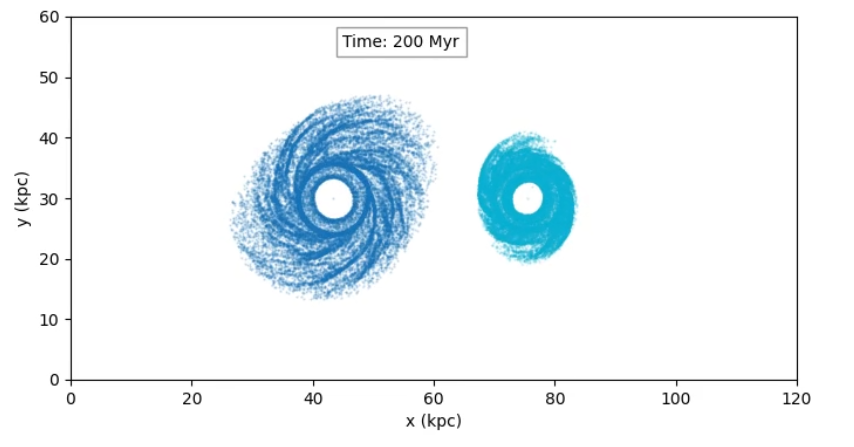
\includegraphics[width=\textwidth]{chapters/results/img/bh-collision/200myr.png}
        \caption{$t=200\,\text{Myr}$}
        \label{fig:collision-bh-sub1}
    \end{subfigure}

    \vspace{0.2cm}

    \begin{subfigure}[b]{0.8\textwidth}
        \centering
        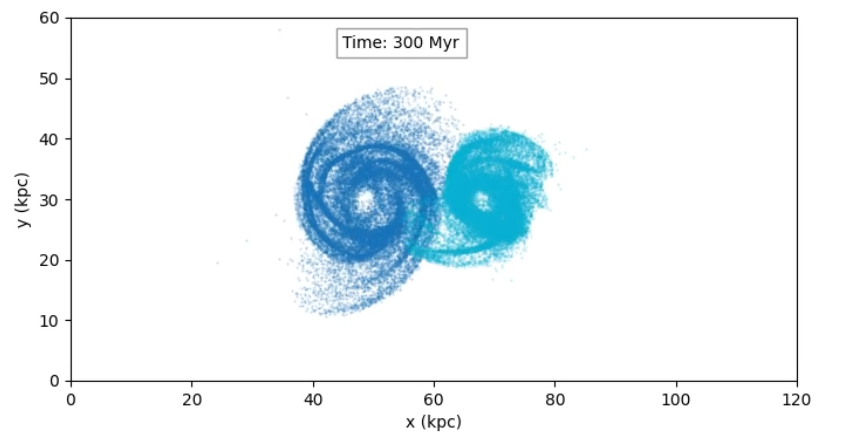
\includegraphics[width=\textwidth]{chapters/results/img/bh-collision/300myr.png}
        \caption{$t=300\,\text{Myr}$}
        \label{fig:collision-bh-sub2}
    \end{subfigure}

    \vspace{0.2cm}

    \begin{subfigure}[b]{0.8\textwidth}
        \centering
        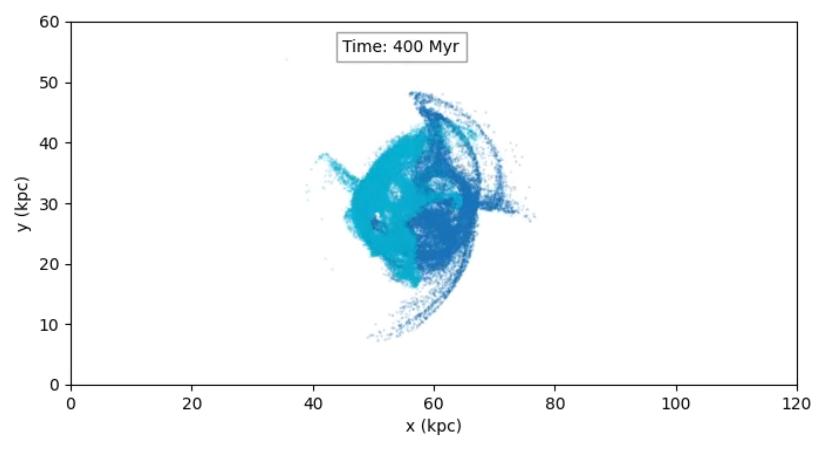
\includegraphics[width=\textwidth]{chapters/results/img/bh-collision/400myr.png}
        \caption{$t=400\,\text{Myr}$}
        \label{fig:collision-bh-sub3}
    \end{subfigure}

    \caption{Galaxy collision stage (Barnes-Hut algorithm).}
    \label{fig:collision-bh}
\end{figure}
Plots of momentum, angular momentum, and energy are shown in \autoref{fig:physical-quantities-bh-collision}.
\begin{figure}[!ht]
    \centering
    \begin{subfigure}[b]{0.45\textwidth}
        \centering
        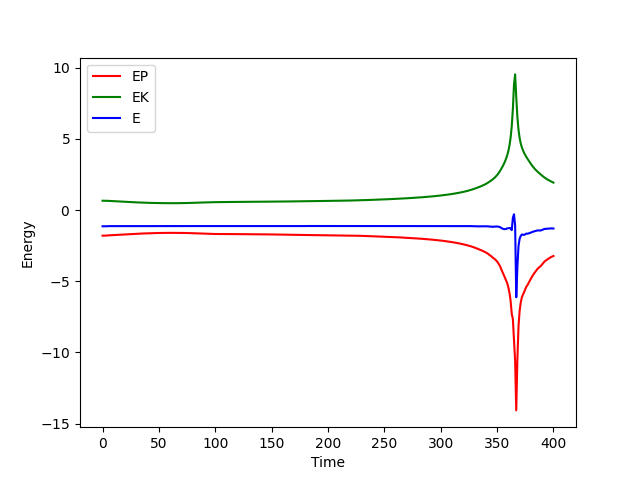
\includegraphics[width=\textwidth]{chapters/results/img/bh-collision/energy.png}
        \caption{Energy}
        \label{fig:physical-quantities-bh-collision-sub1}
    \end{subfigure}
    \hfill
    \begin{subfigure}[b]{0.45\textwidth}
        \centering
        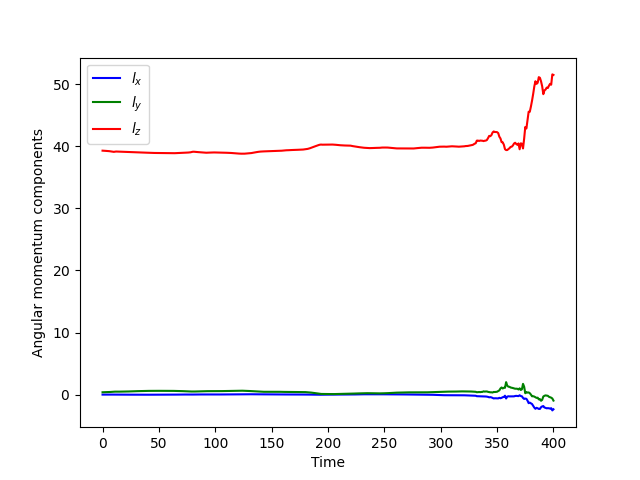
\includegraphics[width=\textwidth]{chapters/results/img/bh-collision/angular-momentum.png}
        \caption{Angular momentum}
        \label{fig:physical-quantities-bh-collision-sub2}
    \end{subfigure}

    \vspace{0.2cm}

    \begin{subfigure}[b]{0.45\textwidth}
        \centering
        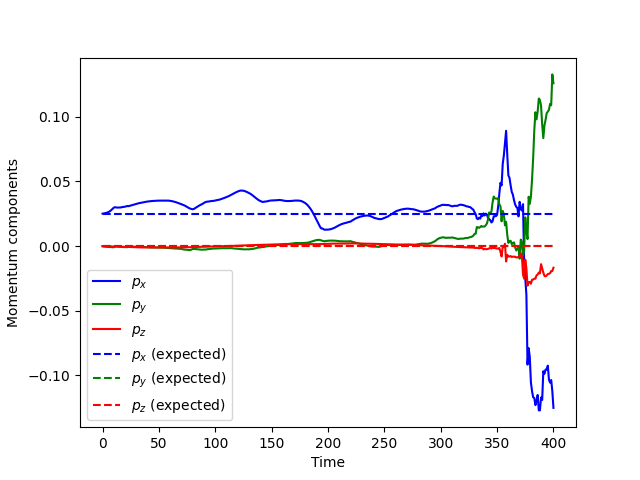
\includegraphics[width=\textwidth]{chapters/results/img/bh-collision/momentum.png}
        \caption{Momentum; broken lines represent the expected momentum following \autoref{eq:expected-momentum-change}}
        \label{fig:physical-quantities-bh-collision-sub3}
    \end{subfigure}

    \caption{Fundamental physical quantities describing the system over time in the Barnes-Hut algorithm.
        Time is in Myr, and the quantities are expressed in units consistent with \autoref{tab:galaxy-parameters}}
    \label{fig:physical-quantities-bh-collision}
\end{figure}

As shown in \autoref{fig:physical-quantities-bh-collision-sub1}, the total energy remains nearly constant until the centers of the two galaxies approach each other closely. At this stage, substantial numerical errors are likely introduced, resulting in a sharp discontinuity between the $t = 350$ Myr and $t = 400$ Myr timestamps.
Around this point, the angular momentum also ceases to be conserved.
Interestingly, the system's momentum oscillates around the expected value throughout the simulation, with the $x$-component displaying the most pronounced deviations.
This behavior reflects the fact that the Barnes-Hut algorithm does not strictly conserve momentum, as the interparticle forces calculated in the Barnes-Hut scheme do not follow Newton's third law.
We conclude by pointing out that the violation of the laws of physics during the collision renders the results collected after this point unreliable.

\subsection{P3M method}
The configuration of the algorithm is the same as in the case of a single galaxy (\autoref{tab:p3m-method-parameters}).
Plots of the physical quantities under consideration are displayed in \autoref{fig:physical-quantities-p3m-collision}, and snapshots from the simulations are shown in \autoref{fig:collision-p3m}.
The figures show that the momentum is conserved for the entire duration of the simulation (\autoref{fig:physical-quantities-p3m-collision-sub3}) and that there is a slight jump in the components of the angular momentum between 300 and 400 Myrs (\autoref{fig:physical-quantities-p3m-collision-sub2}), corresponding to the galaxy centers coming closely together.
The energy plots (\autoref{fig:physical-quantities-p3m-collision-sub1}) roughly match the energy plots in the Barnes-Hut method (\autoref{fig:physical-quantities-bh-collision-sub1}).
However, the potential energy (and, as a consequence, the total energy) oscillates irregularly during the simulation.
A probable source of this phenomenon is the inaccuracy in representing the very deep potential well generated by the massive particle in the center of the galaxy by the potential mesh.
This leads to fluctuations as the massive particle moves across the grid.
However, a more in-depth study would need to be undertaken to find a definitive explanation.

\subsection{PM method}
The method's configuration remains the same as in the single galaxy simulation (\autoref{tab:pm-method-parameters}).
Plots of the physical quantities under consideration are displayed in \autoref{fig:physical-quantities-pm-collision}, and snapshots from the simulations are shown in \autoref{fig:collision-pm}.
The deviations of the momentum and angular momentum components from their initial values (\autoref{fig:physical-quantities-pm-collision-sub2} and \autoref{fig:physical-quantities-pm-collision-sub3}) are greater compared to the \PThreeM{} method.
Additionally, the oscillations in the potential and total energies are significant, raising serious doubts about whether the simulation can be accepted as physically valid.
Examination of the system at $t = 200$ and $300$ Myr (\autoref{fig:collision-pm-sub1} and \autoref{fig:collision-pm-sub2}) reveals that the interactions between the galactic center and the surrounding disk particles are not accurately captured.
The central `hole'' in the disk begins to vanish as nearby particles collapse inward.
In contrast, the Barnes-Hut (\autoref{fig:collision-bh-sub1}, \autoref{fig:collision-bh-sub2}) and \PThreeM{} (\autoref{fig:collision-p3m-sub1}, \autoref{fig:collision-p3m-sub2}) simulations at the same time points maintain a well-defined circular hole.